% BEGIN PREAMBEL
\documentclass[9pt]{beamer}
\usepackage[british]{babel}
\usepackage[latin1]{inputenc}
\usepackage{multimedia}
\usepackage{amsmath,amsfonts,amssymb}
\usepackage{upgreek}
\usepackage{pgfpages}
\usepackage[version=3]{mhchem}
\usepackage{lmodern}
\usepackage{graphicx}
\usepackage{multicol}
\usepackage{xcolor}
\usepackage{wrapfig}
\usepackage{siunitx}
\newcommand{\as}{\\[14pt]}
\newcommand{\s}{\\[7pt]}
\newcommand{\is}{\\[2pt]}
\newcommand{\no}{\noindent}
\newcommand{\ka}{\hspace*{0.5cm}}
\newcommand{\ma}{\hspace*{1cm}}
\newcommand{\ga}{\hspace*{1.5cm}}
\newcommand{\li}{\left|}
\newcommand{\re}{\right|}
\newcommand{\const}{\text{const.}}
\newcommand{\z}{\text}
\newcommand{\terminal}[1]{\colorbox{black}{\textcolor{white}{{\fontfamily{phv}\selectfont \scriptsize{#1}}}}}
\newcommand{\plugin}[1]{\textit{\flq#1\frq}}
\usetheme{Boadilla}
\graphicspath{ {Pics/} }
\usecolortheme{beaver}
\useoutertheme{miniframes}
\beamertemplatenavigationsymbolsempty
\makeindex
\title[Layer1 Module Soft]{Software Upgrade for the CMS Layer1 Module}
\author[M. Reichmann]{Michael Reichmann}
\institute[\textbf{\textit{ETH}}\scalebox{.6}{\textit{Z\"{u}rich}}]{Swiss Federal Institute of Technology Zurich}
\AtBeginSection{\frame{\sectionpage}}
% END PREAMBEL
\begin{document}
% ============================
% BEGIN TITLE PAGE
% ============================
\begin{frame}
	\begin{center}
		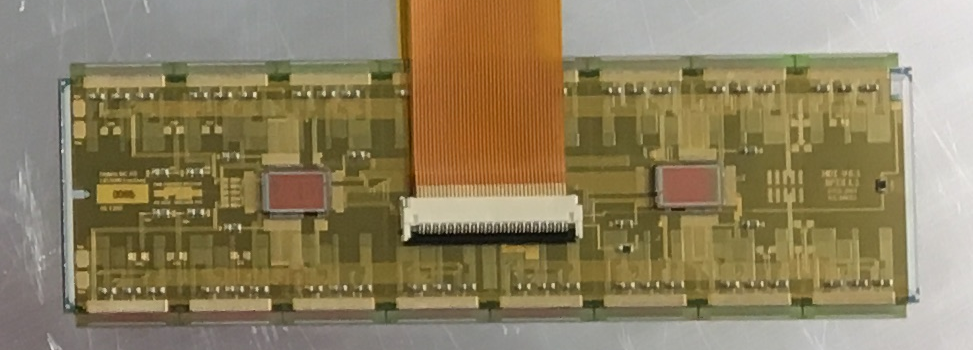
\includegraphics[width=8cm]{Mod}
	\end{center}
	\begin{alertblock}{
		\begin{center}
			\textbf{Software Upgrade for the CMS Layer1 Module}
		\end{center}}
		\vspace*{10pt}
		\begin{center}\small
		Michael Reichmann
		\end{center}\normalsize
	\end{alertblock}
\end{frame}
% END
% ============================
% BEGIN TABLE OF CONTENTS
% ============================
\begin{frame}[allowframebreaks]
	\frametitle{Table of contents}
	\tableofcontents   % [pausesections]
\end{frame}
% END
% ====================================================================================
% BEGIN MOTIVATION
% ====================================================================================
\section{Motivation}
% ============================
\begin{frame}
	\begin{itemize}
		\setlength{\itemsep}{\fill}
		\item tracker has to handle larger amount of data
		\begin{itemize}
			\item $50$ instead of $25$ collisions per bunch crossing after the next upgrade
		\end{itemize}
		\item adding innermost layer to the CMS tracker with a new module design (highest data volume)
		\begin{itemize}
			\item equipped with new PROC600 as ROC $\rightarrow$ higher data processing speed
		\end{itemize}
		\item current modules currently work with one TBM which has two SDATA lines
		\begin{itemize}
			\item $8$ ROCs per line
		\end{itemize}
		\item improve readout speed by adding a second TBM
	\end{itemize}
\end{frame}
% END MOTIVATION
% ====================================================================================
% BEGIN LAYOUT
% ====================================================================================
\section{Layout}
% ============================
\subsection{Schematics}
\begin{frame}
	\begin{center}
		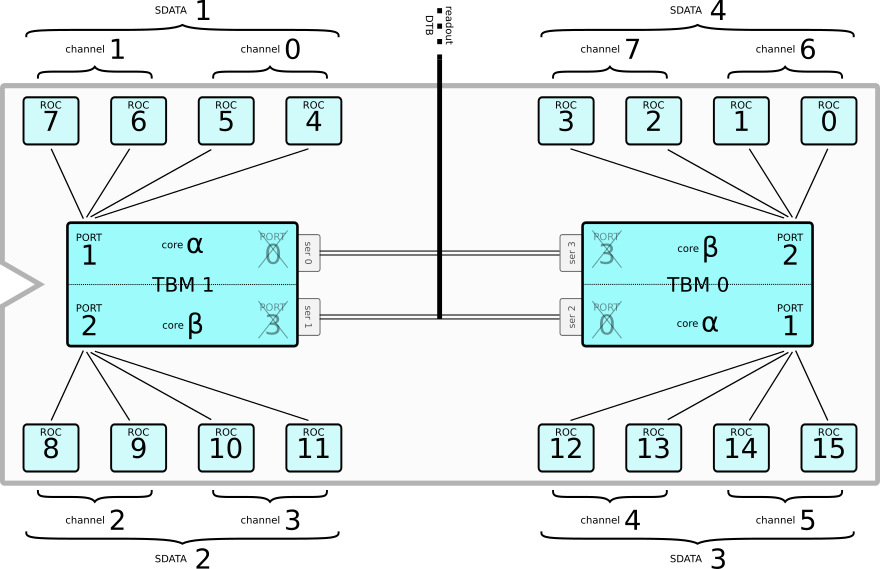
\includegraphics[width=\textwidth]{Schematics}
	\end{center}
\end{frame}
% ============================
\subsection{Digital Module Adapter}
\begin{frame}
	\begin{itemize}
		\setlength{\itemsep}{\fill}
		\item adapter from Molex of the module to the SCSI of the DTB
		\item old module has a Molex connector for a $33$ pin cable
		\item additional TBM requires additional lines
		\begin{itemize}
			\item two pairs of differential SDATA lines
			\item one pair of RDA lines (for TBM feedback)
			\item pin for shielding
			\item one VD+ less
		\end{itemize}
		\item Molex connector of the Layer1 module has $39$ pins
		\item new adapter design by Martin Lickteig
	\end{itemize}
	\begin{minipage}{5.5cm}
		\centering
		\includegraphics[width=5cm]{digAdapter}
	\end{minipage}
	\hspace*{2pt}
	\begin{minipage}{5.5cm}
		\centering
		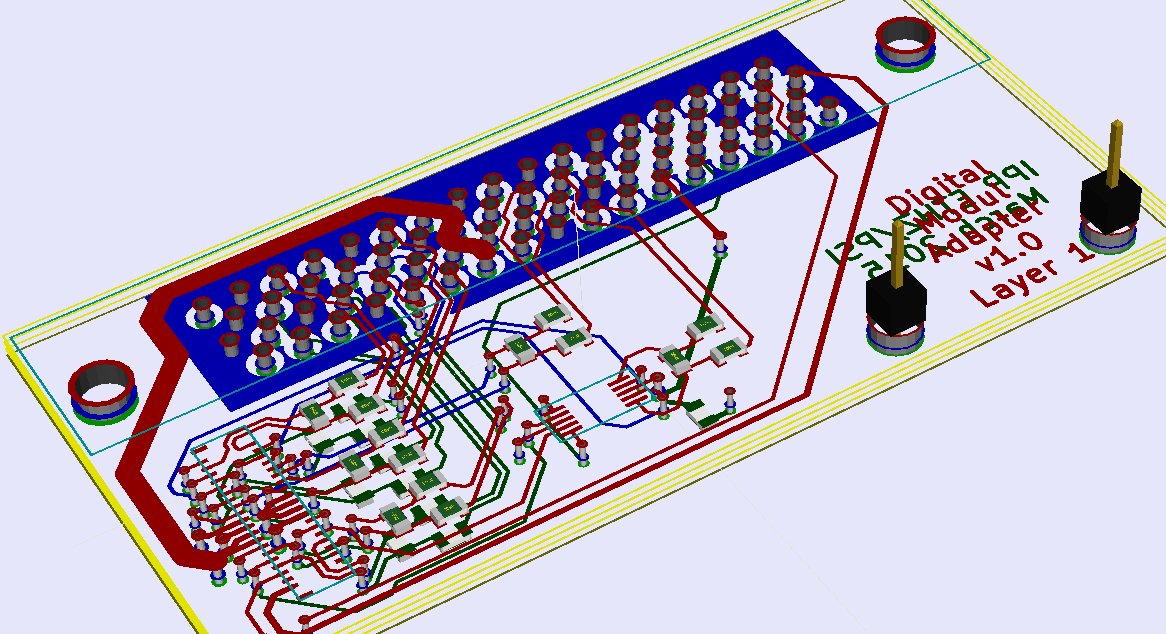
\includegraphics[width=5cm]{digAdapter3D}
	\end{minipage}
\end{frame}
% new frame ===================
\begin{frame}
	\begin{center}
		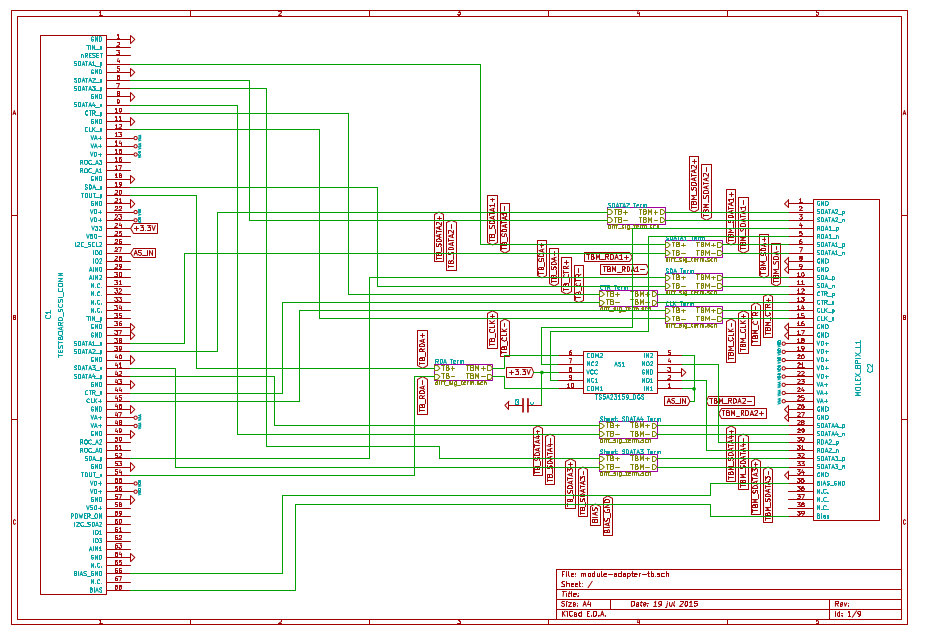
\includegraphics[width=0.95\textwidth]{connector}
	\end{center}
\end{frame}
% END LAYOUT
% ====================================================================================
% BEGIN TEST MODULES
% ====================================================================================
\section{Modules for Testing}
% ============================
\begin{frame}
	\underline{\textbf{Currently available:}}
	\begin{itemize}
		\setlength{\itemsep}{\fill}
		\item PSI produced two layer1-like modules based on bare dig2.1respin modules:
		\begin{itemize}
			\item one with TBM09 (current Token Bit Manager)
			\item one with the new TBM10 $\rightarrow$ electrical shortcut
			\begin{itemize}
				\item sensors cannot be biased
			\end{itemize}
		\end{itemize}
	\end{itemize}
	\vspace*{1cm}
	\underline{\textbf{TMB10:}}
	\begin{itemize}
		\setlength{\itemsep}{\fill}
		\item TBM10 has additional delay of three clock cycles between trigger and token
		\begin{itemize}
			\item required by PROC600
		\end{itemize}
	\end{itemize}
	\vspace*{1cm}
	\underline{\textbf{Plan on further modules:}}
	\begin{itemize}
		\item fully working module with TBM10 and digv2.1respin (no shortcut)
		\item module with PROC600 as soon as new chip iteration is produced
	\end{itemize}
\end{frame}
% new frame ===================
\begin{frame}
	\begin{center}
		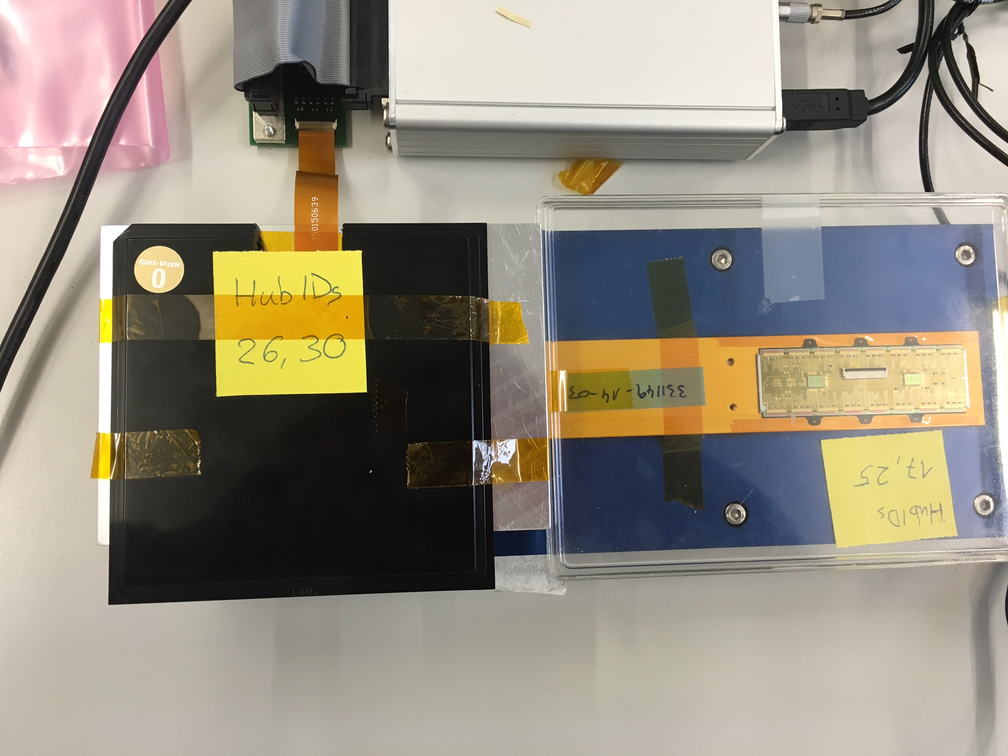
\includegraphics[height=0.85\textheight]{bothMod}
	\end{center}
\end{frame}
% END TEST MODULES
% ====================================================================================
% ====================================================================================
% BEGIN DTB 
% ====================================================================================
\section{Changes of the DTB}
% ============================
\subsection{Software}
\begin{frame}
	\frametitle{C\texttt{++} code accessed by pXar on a virtual processor on the FPGA}
	\underline{\textbf{Issues:}}
	\begin{itemize}
		\setlength{\itemsep}{\fill}
		\item ROC I$^{2}$C addresses remain the same
		\item HubIDs (hard wired address of the TBM) and PortAddresses change
	\end{itemize}
	\vspace*{10pt}
	\underline{\textbf{Software Additions:}}
	\begin{itemize}
		\setlength{\itemsep}{\fill}
		\item \ubu{bool layer1}: adding boolean as identifier for the layer1 module
		\item \ubu{void roc\_I2cAddr\_Layer\_1(uint8\_t id)}: sets the correct HubAddress for layer1
		\item \ubu{const unsigned char CTestboard::MODCONF L1[16]}: stores the port addresses
		\item \ubu{void mod\_Addr(uint8\_t hub0, uint8\_t hub1)}: accessible in pXar, sets the HubIDs
	\end{itemize}
\end{frame}
% ============================
\subsection{Firmware}
\begin{frame}
	\frametitle{Verilog FPGA design}
	\underline{\textbf{Issue:}}
	\begin{itemize}
		\item only $3$ Deserializer400 implemented
		\begin{itemize}
			\item due to former compiling issues
		\end{itemize}
	\end{itemize}
	\vspace*{10pt}
	\underline{\textbf{Changes:}}
	\begin{itemize}
		\item reactivation of the 4th Deserializer400 to handle the 4 data streams
	\end{itemize}
\end{frame}
% END DTB
% ====================================================================================
% BEGIN PXAR 
% ====================================================================================
\section{Changes in PXAR}
% ============================
\subsection{Additional TBM}
\begin{frame}
	\begin{itemize}
		\item \ubu{tbmConfig} in pXar almost built up correctly by module parameters in configuration file
		\begin{itemize}
			\item \ubu{nModules, nRocs, nTBMs}
			\item rename \ubu{tbmConfig} to \ubu{tbmCoreConfig}
		\end{itemize}
	\end{itemize}
	\vspace*{10pt}
	\underline{\textbf{Issue:}}
	\begin{itemize}
		\item cannot handle more than one HubID 
	\end{itemize}
	\vspace*{10pt}
	\underline{\textbf{Solution:}}
	\begin{itemize}
		\item changing \ubu{usigned int fHubId} to \ubu{vector<uint8\_t> fHubIds}
	\end{itemize}

\end{frame}
% END PXAR
% DOCUMENT END
\end{document}

